%%
\subsection*{Model} \label{sec:model}

We model the microbial abundances across time along the lines of Blumm \textit{et al.}\cite{ranking}. The dynamics of taxon relative abundances is described by the Langevin equation:
\begin{linenomath}
\begin{equation}
\dot{x_i} = F_i \cdot x_i^\alpha + V \cdot x_i^\beta \xi_i(t) - \phi(t) \cdot x_i,
\end{equation}
\end{linenomath}
where F$_i$ captures the fitness of the taxon i, V corresponds to the noise amplitude and $\xi_i$(t) is a Gaussian random noise with zero mean  $<\xi_i(t)>$ = 0 and variance uncorrelated in time, $<\xi_i(t) \xi_i(t')>$ =  $\delta(t'-t)$, . The function $\phi(t)$ ensures the normalization at all times, $\sum x_i(t) = 1$, and corresponds to $\phi(t) = \sum F_i x_i^\alpha + \sum V x_i^\beta \xi_i(t)$.
The temporal evolution of the probability that a taxon i has a relative abundance $x_i(t)$, P(x$_i$,t), is determined by the Fokker-Planck equation:
\begin{linenomath}
\begin{equation}
\frac{\partial P}{\partial t} = - \frac{\partial}{\partial x_i}  [(F_i \cdot x_i^\alpha - \phi(t) \cdot x_i ) \cdot P]+ \frac{1}{2} \frac{\partial^2}{\partial x_i^2} (V^2 \cdot x_i^{2\beta}\cdot P).
\end{equation}
\end{linenomath}
The microbiota evolves towards a steady-state with a time-independent probability depending on the values of $\alpha$, $\beta$, F$_i$ and V. For $\alpha<1$ (otherwise, systems are always unstable), the steady-state probability may be localized in a region around a preferred value or broadly distributed over a wide range, depending on whether the fitness F$_i$  dominates or is overwhelmed by the noise amplitude V. The steady-state solution of the Fokker-Planck equation is given by:
\begin{eqnarray}
P_0 (x_i) &=& C_{ne}(\alpha,\beta,F_i,V)  \cdot x_i^{-2\beta}  \cdot \exp\Big[\frac{2F_i}{V^2}\frac{x_i^{1+\alpha-2\beta}}{1+\alpha-2\beta}-\frac{\phi_0}{V^2}\frac{x_i^{2-2\beta}}{1-\beta}\Big] \quad \textrm{if} \quad  2\beta \ne 1+\alpha, \notag \\
P_0 (x_i) &=& C_e(\alpha,\beta,F_i,V)  \cdot x_i^{\frac{2F_i}{V^2} -2\beta}  \cdot \exp\Big[\frac{\phi_0}{V^2}\frac{x_i^{2-2\beta}}{1-\beta}\Big] \quad \textrm{if} \quad  2\beta = 1+\alpha,
\notag
\end{eqnarray}
where $\phi_0 = (\sum_i F_i^{1/(1-\alpha)})^{1-\alpha}$ and C$_{ne}$ and C$_{e}$ are integrals that should be solved numerically for the parameters of interest. The ordered phase happens when the solution has a maximum in the physical interval ($0<x_i<1$). For larger V, the transition to a disordered phase happens when the maximum shifts to the unphysical region $x_i<0$, which sets the phase transition region V($\alpha,\beta,F_i$). The phase transition region can be calculated analytically in particular cases:
\begin{eqnarray}
F_i^2 &=& 4 \beta \phi_0 V^2\quad \textrm{if} \quad  \beta = \alpha \neq 1, \notag \\
F_i &=& \beta V^2\quad \textrm{if} \quad  2\beta = 1+\alpha,
\notag
\end{eqnarray}
where the first case, simplifies to $F= 3 V^2$ if $\beta = 0.75$ and the fitness of this taxon dominates in $\phi_0$. 
In many physical systems (Brownian motion is the classical example), the two terms of the Langevin equation are related.  The \emph{fluctuation--dissipation theorem} states a general relationship between the response to an external disturbance and the internal fluctuations of the system\cite{FD}. The theorem can be used as the basic formula to derive the fitness from the analysis of fluctuations 
of the microbiota, assuming that it is in equilibrium (the ordered phase).  

\todo{Explain better the fluctuation-dissipation theorem}


%%
\subsection*{Selection and Methods}

The bacteria and archaea taxonomic assignations were obtained by analysing 16S rRNA sequences, which were clustered into operational taxonomic units (OTUs) sharing 97 \% sequence identity using QIIME\cite{QIIME}. WGS data\cite{kwashiorkor} were analysed and assigned at strain level by the Livermore Metagenomic Analysis Toolkit (LMAT)\cite{LMAT}, according to their default quality threshold. Genus, with best balance between error assignment and number of taxa, was chosen as our reference taxonomic level. We have verified that our conclusions are not significantly affected by selecting family or species as the reference taxonomic level (see Figure \ref{fig:taxlev1}).

%%
\subsubsection*{Sample selection}
We have chosen studies about relevant pathologies containing metagenomic sequencing time data series of bacterial populations from humans in different healthy and non-healthy states. We have selected only those individuals who had three or more time points of data available in databases. Caporaso et al. study \cite{moving} was selected as it has two healthy individuals measured over a very large timespan, with almost daily sampling. Faith et al. study \cite{LEA} was selected due to the BMI differences between subjects, moreover some of them had diets which can be treated as system perturbations. We considered healthy only those individuals who had normal or overweight BMI. Smith et al., study \cite{kwashiorkor} was selected for both the age of the patients and the rare disease. We only worked with the discordant twins, and considered healthy those who were not affected by kwashiorkor in each pair of patients. David et al., study \cite{diet} was selected for its differential diets. We considered as the healthy part the first time samples of each individual before the diet, and the rest of time points as perturbations. Dethlefsen and Relman work \cite{antibiotics} was selected due to the interesting treatment of two antibiotic intakes of the same antibiotic by three different subjects. We considered as the healthy part only those times before any antibiotic treatment, and as perturbations the time of antibiotic intakes and the period after that. And finally, we also considered a study made in our group carried by Durb�n et al., \cite{IBS} in which we considered as healthy subjects those who didn't suffer from irritable bowel disease, and as perturbation the patients who had this disease. 

Metadata of each study is provided in Tables \ref{tab:diet} to \ref{tab:LEA}. All used 16S rRNA gene sequencing except for the study of the discordant kwashiorkor twins\cite{kwashiorkor} (see Tables \ref{tab:DH} and \ref{tab:DK}) where shotgun metagenomic sequencing (SMS) and 16S rRNA were used. In the latter case we selected to work with SMS data to show that our method is valid regardless of the source of taxonomic information. Each one of the datasets was treated as follows:

%%
\subsubsection*{16rRNA sequences processing}
Reads from the selected studies were first quality filtered using the FastX toolkit\cite{FASTX}, allowing only those reads which had more than 25 of quality along the 75\% of the complete sequence. 16S rRNA reads were then clustered at 97\% nucleotide sequence identity (97\% ID) into operational taxonomic units (OTUs) using QIIME package software\cite{QIIME} (version 1.8) We followed open reference OTU picking workflow in all cases. The clustering method used was uclust, and the OTUs were matched against Silva database\cite{SILVA} (version 111, July 2012) and were assigned to taxonomy with an uclust-based consensus taxonomy assigner. The parameters used in this step were: similarity 0.97, prefilter percent id 0.6, max accepts 20, max rejects 500. 

%%
\subsubsection*{Metagenomic sequences processing}
Metagenomic shotgun (and 16S too) sequences were analyzed with LMAT (Livermore Metagenomics Analysis Toolkit) software package\cite{LMAT} (version 1.2.4, with Feb'15 release of data base \emph{LMAT-Grand}). LMAT was run using a Bull shared-memory node belonging to the team's HPC (high performance computing) cluster. It is equipped with 32 cores (64 threads available using Intel Hyper-threading technology) as it has two Haswell-based Xeons ($22\un{nm}$ technology), the E5-2698v3@2.3 GHz, sharing half a tebibyte (0.5 TiB, that is, 512 gibibytes) of DRAM memory. This node is also provided with a PCIe SSD card as NVRAM, the Micron P420m HHHL, with 1.4 TB, and 750000 reading IOPS, 4 KB, achieving 3.3 GB/s. The computing node was supplied with a RAID-0 (striping) scratch disk area. We used the ``Grand'' database\cite{LMAT2}, release Feb'15, provided by the LMAT team, where ``Grand'' refers to a huge database that contains k-mers from all viral, prokaryote, fungal and protist genomes present in the NCBI database, plus Human reference genome (hg19), plus GenBank Human, plus the 1000 Human Genomes Project (HGP) (this represent about 31.75 billion k-mers occupying 457.62 GB)\cite{LMAT2}. Previously to any calculation, the full database was loaded in the NVRAM. With this configuration the observed LMAT sustained sequence classification rate was $20\unclassrate$. Finally, it is worth mentioning that a complete set of Python scripts have been developed as back-end and front-end of the LMAT pipeline in order to manage the added complexity of time series analysis. 

%%
\subsubsection*{Taxa level selection}
We selected genus as taxonomic level for the subsequent steps of our work. In order to ensure that, between adjacent taxonomic levels, there were not crucial differences which could still be of relevance after standardization (see last subsection of Material and Methods), we tested two different data sets. In the former, the antibiotics study\cite{antibiotic} with 16S data, we tested the differences between genus and family levels. The latter dataset tested was the kwashiorkor discordant twins study\cite{kwashiorkor} for both genus and species taxonomic levels. The Figures \ref{fig:taxlev1} (overview) and \ref{fig:taxlev2} (detail) plot the comparison between studies (and so, 16S and SMS) and between adjacent taxonomic levels.

\begin{figure} 
  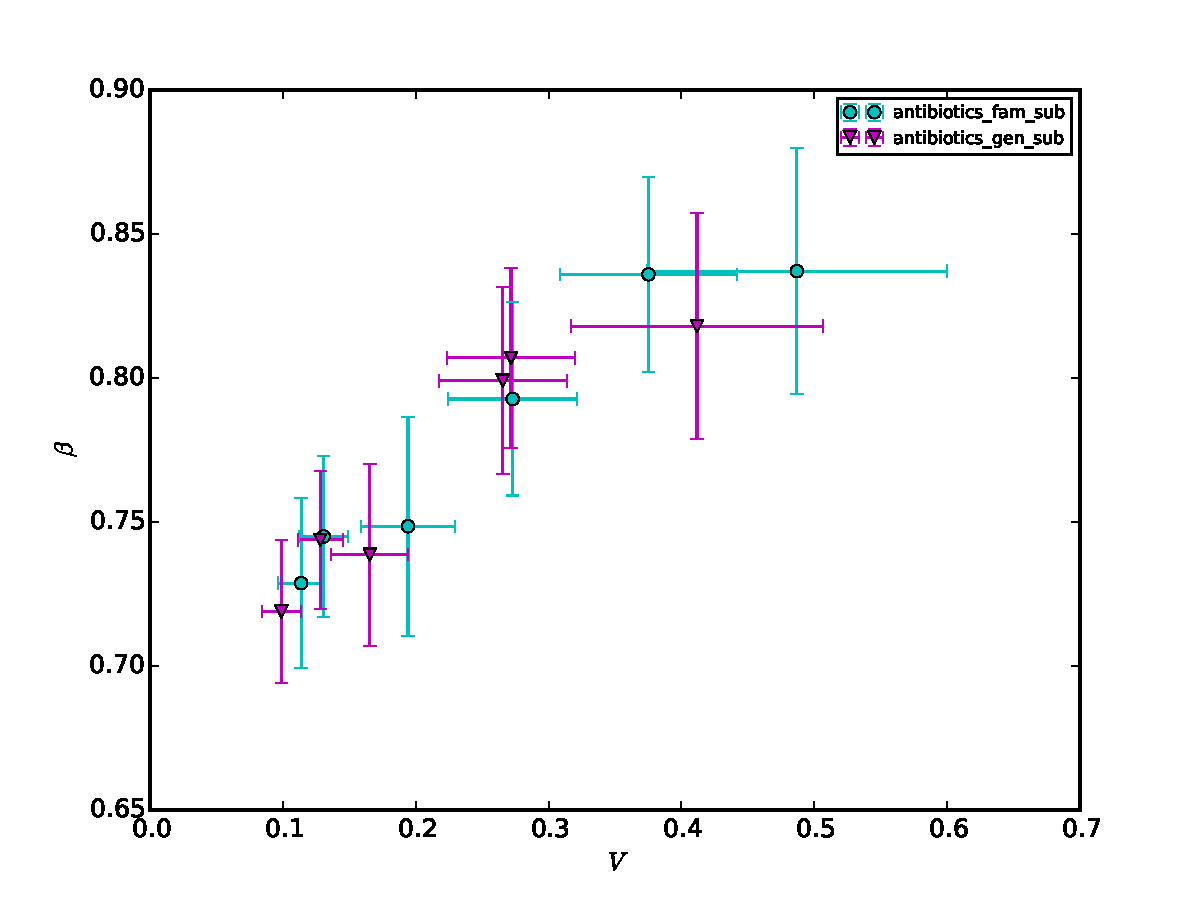
\includegraphics[width=0.5\textwidth]{results/taxalevel/sum_raw_16S.pdf}
  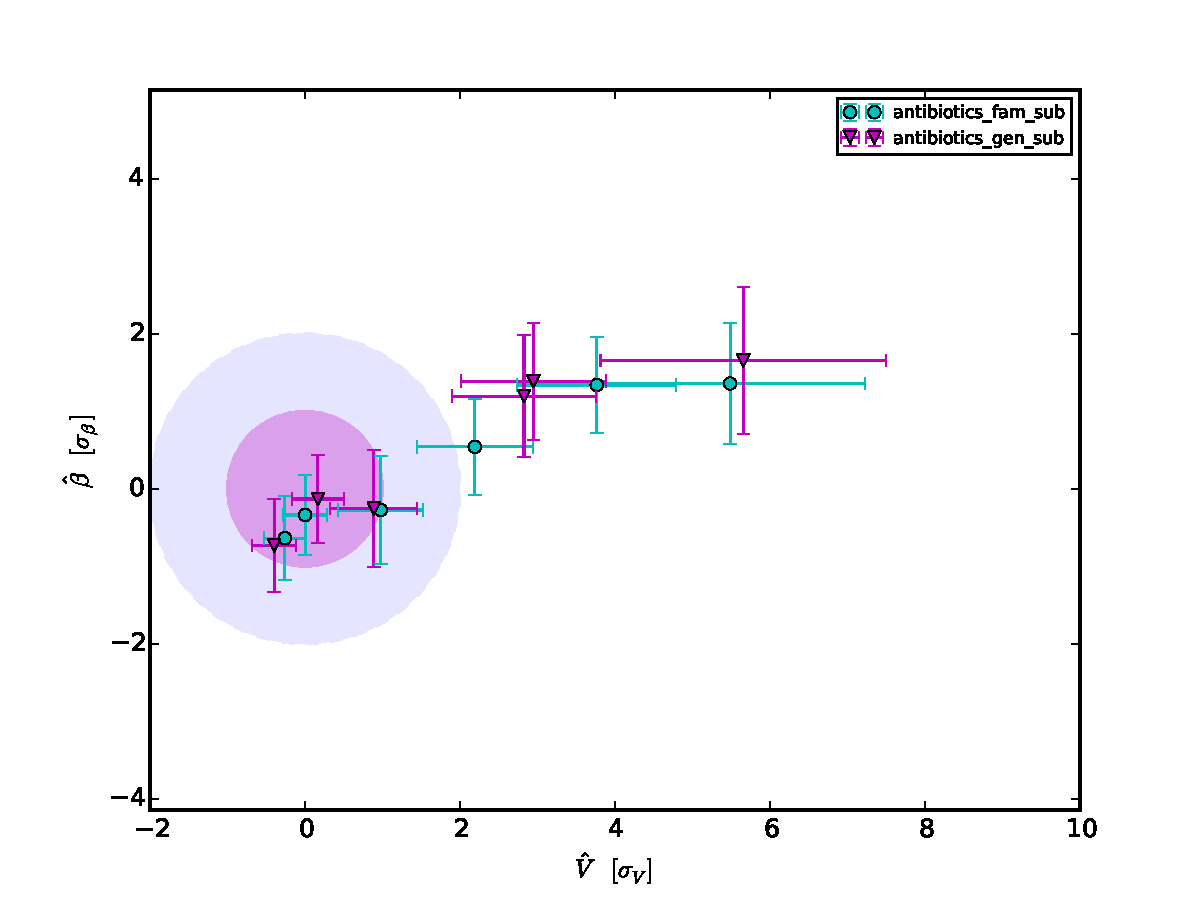
\includegraphics[width=0.5\textwidth]{results/taxalevel/sum_sta_16S.pdf}
  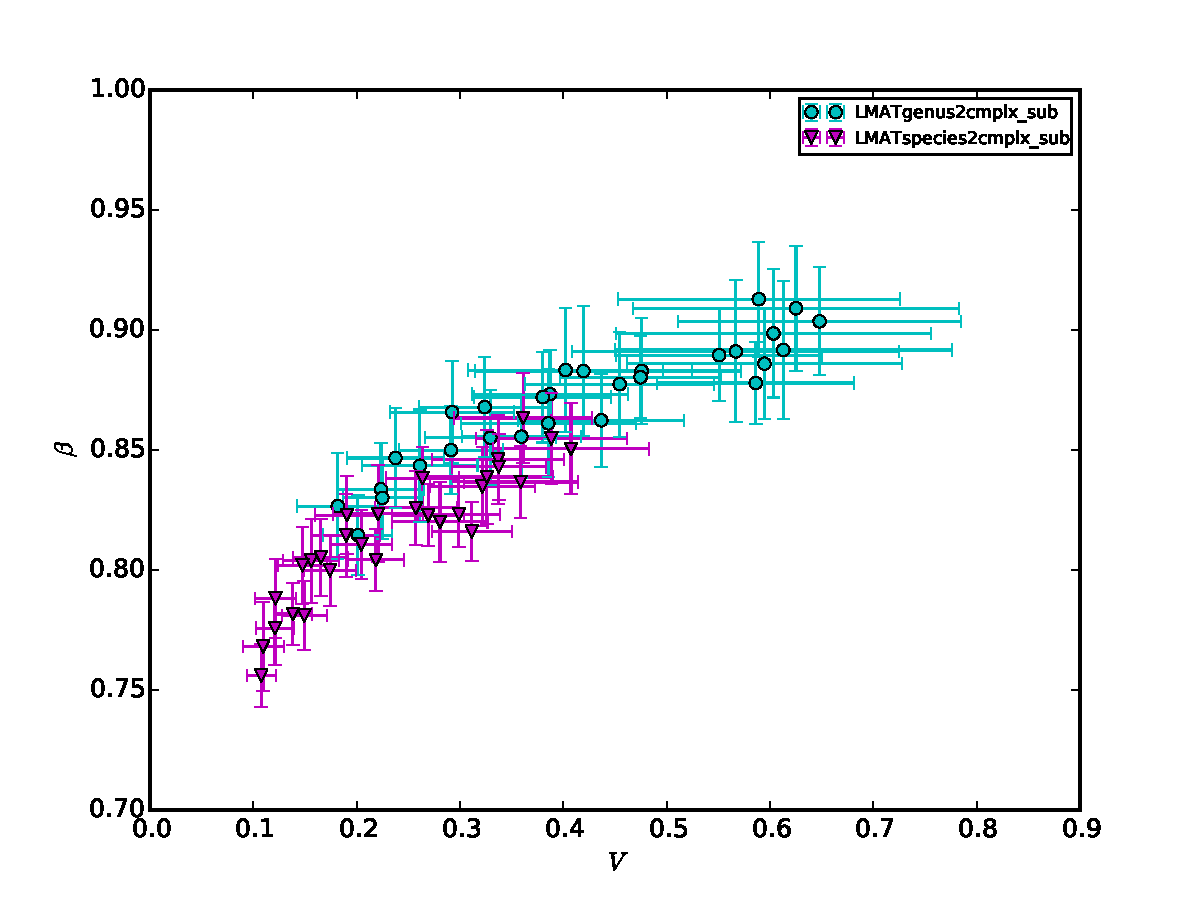
\includegraphics[width=0.5\textwidth]{results/taxalevel/sum_raw_SMS.pdf} 
  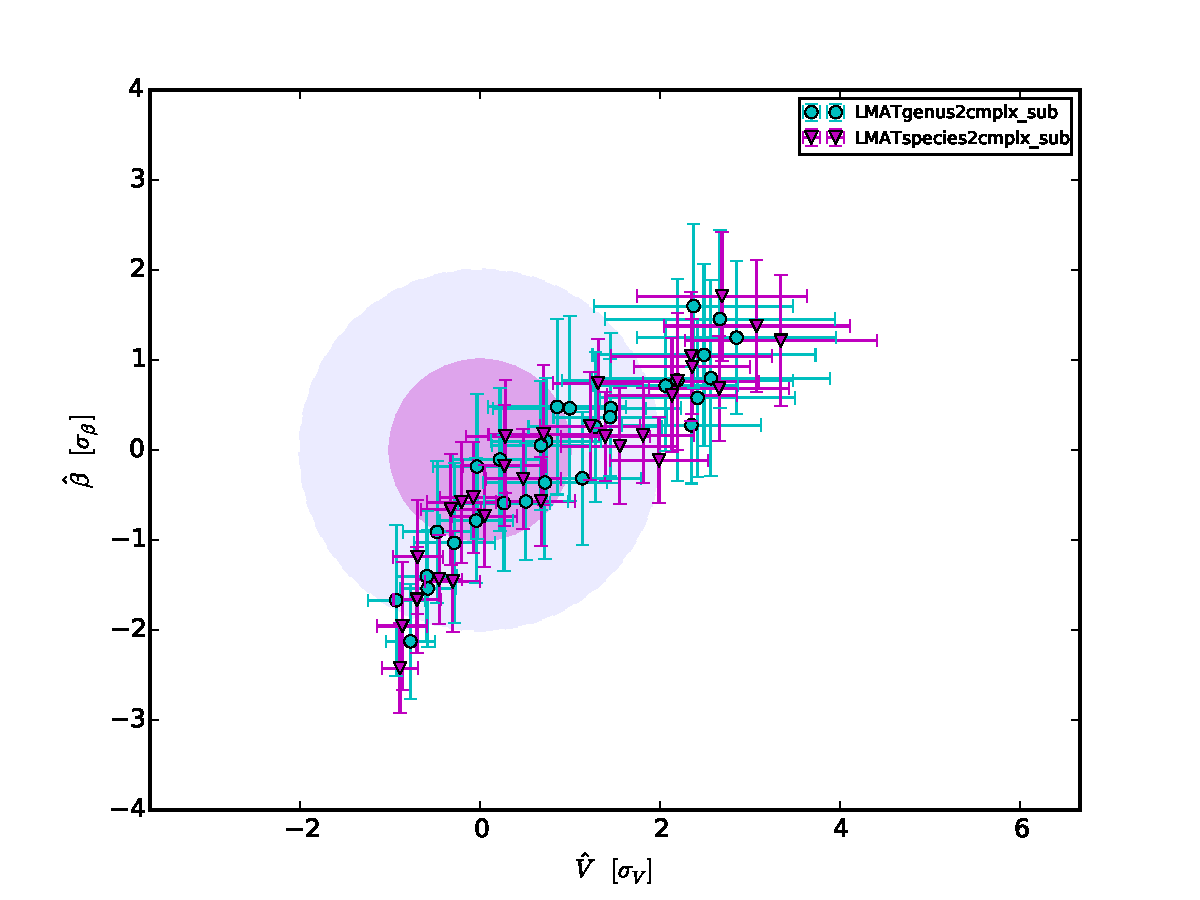
\includegraphics[width=0.5\textwidth]{results/taxalevel/sum_sta_SMS.pdf}
\caption{Overview of comparison of different approaches based on adjacent taxonomic levels using plots in the Taylor-parameters space. For 16S (former row of subfigures), the levels are family vs. genus, whereas for SMS (latter row of subfigures) levels are genus vs. species. The left column shows the raw results and the right column plots the standardized results (see Section \ref{sec:stan})}
\label{fig:taxlev1}
\end{figure}

\begin{figure} 
  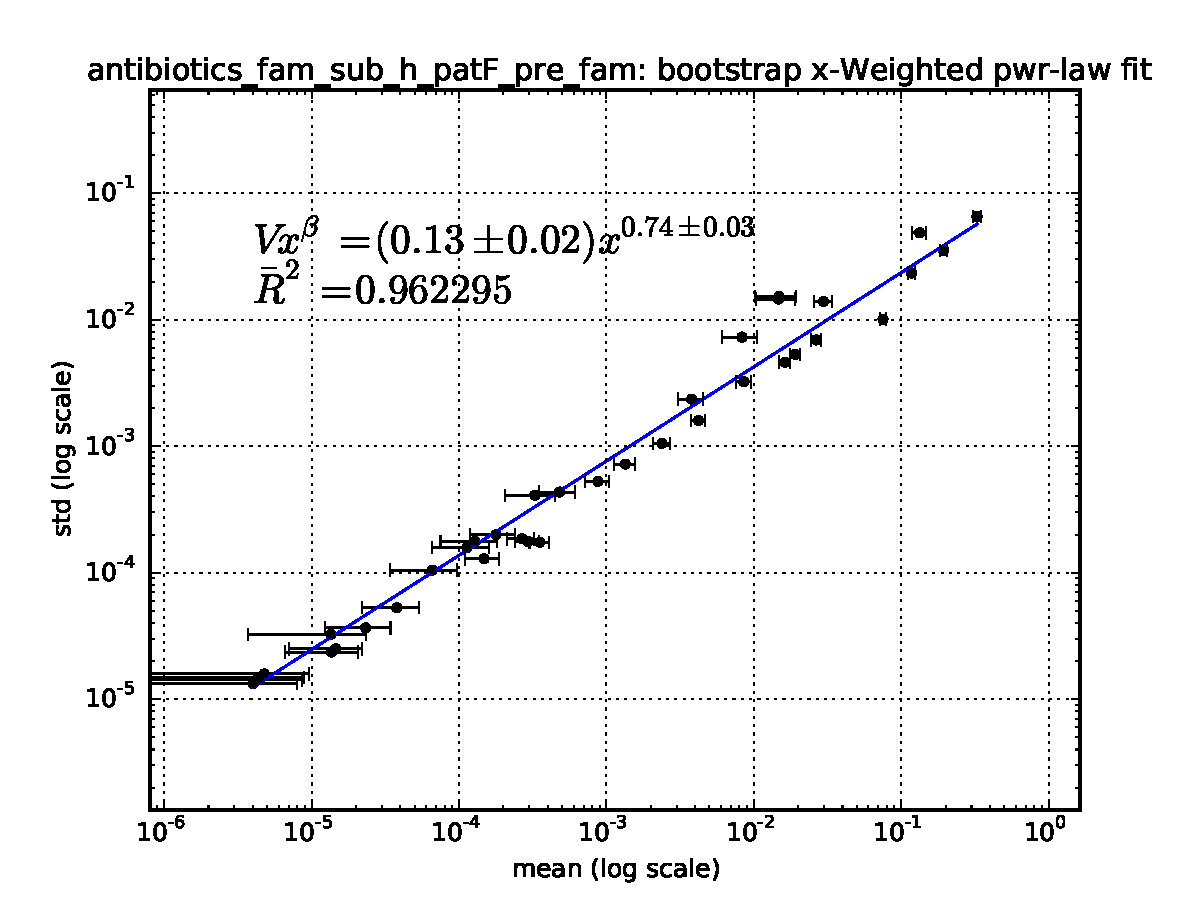
\includegraphics[width=0.5\textwidth]{results/taxalevel/xWb_fam_16S.pdf}
  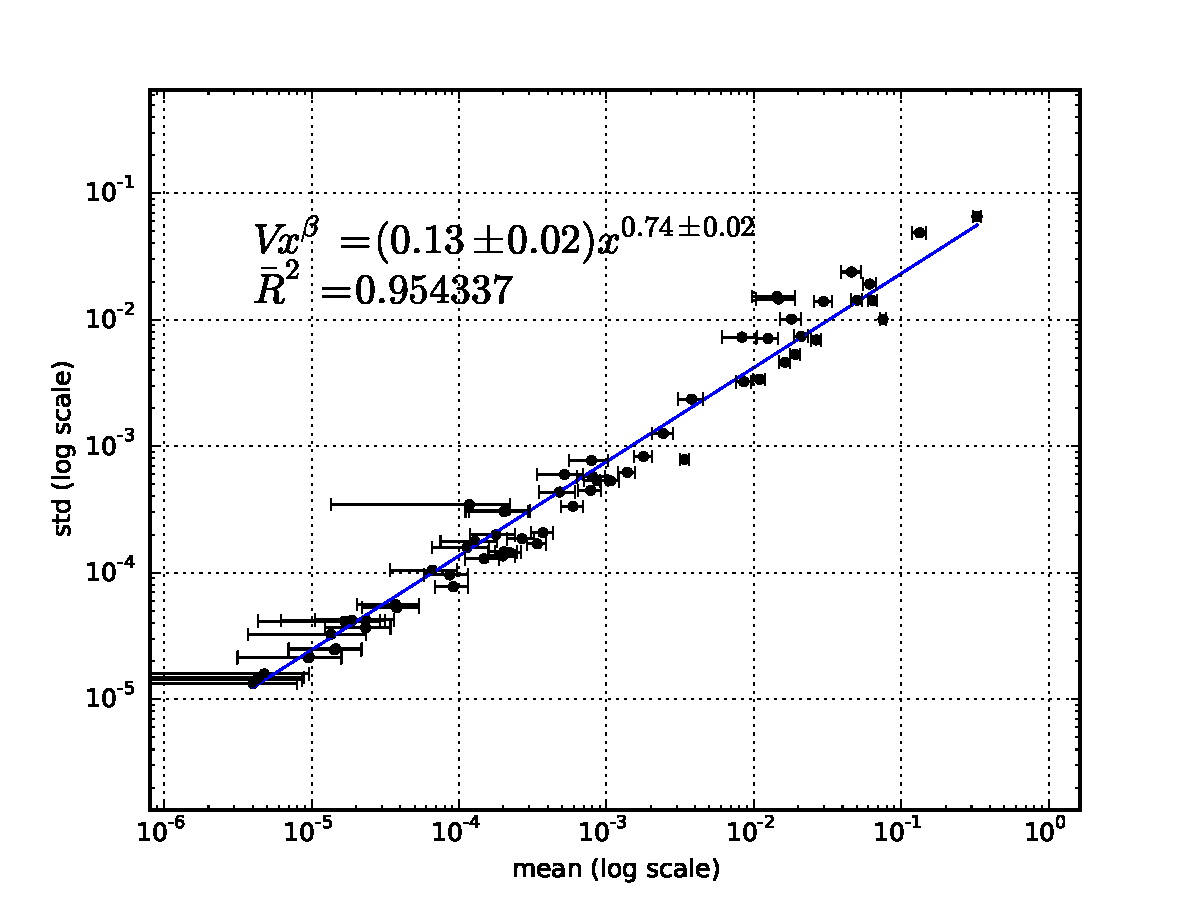
\includegraphics[width=0.5\textwidth]{results/taxalevel/xWb_gen_16S.pdf}
  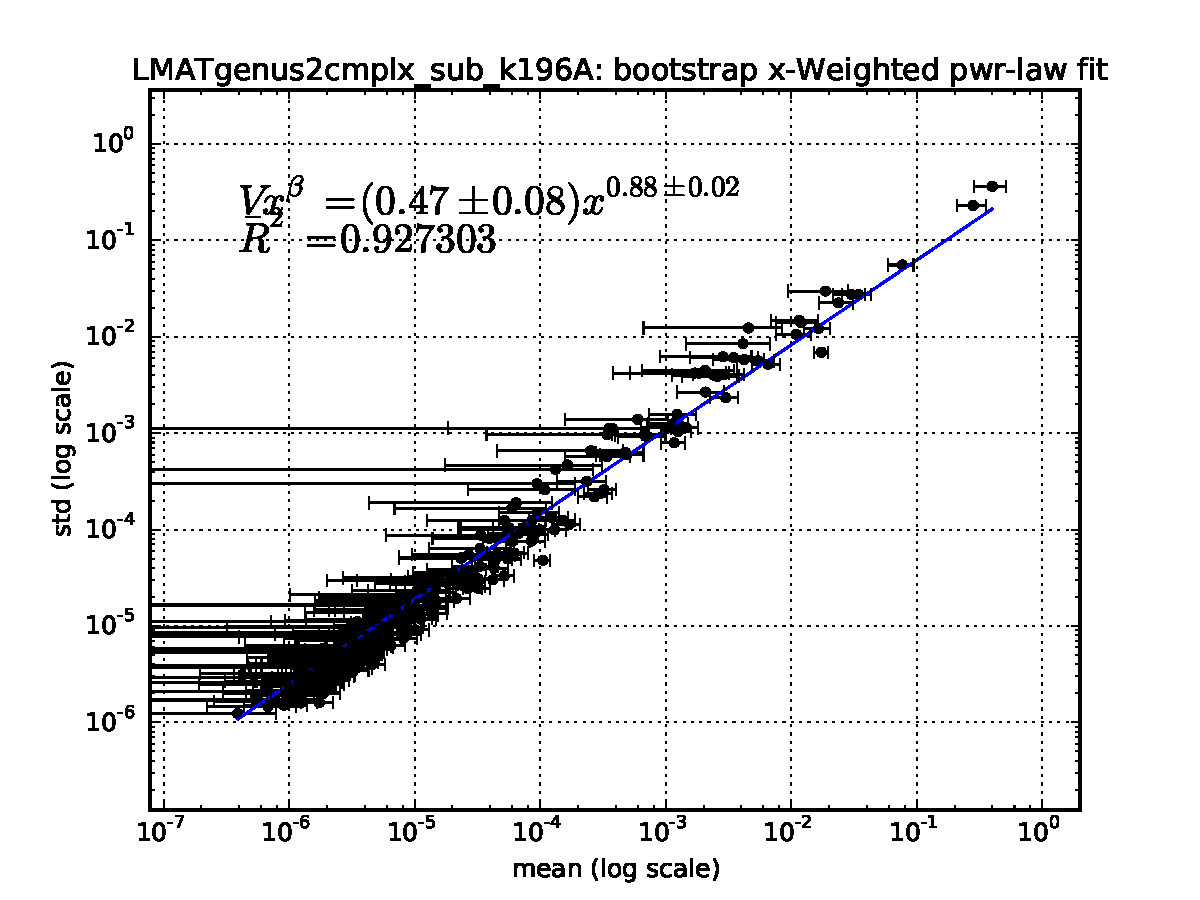
\includegraphics[width=0.5\textwidth]{results/taxalevel/xWb_gen_SMS.pdf}
  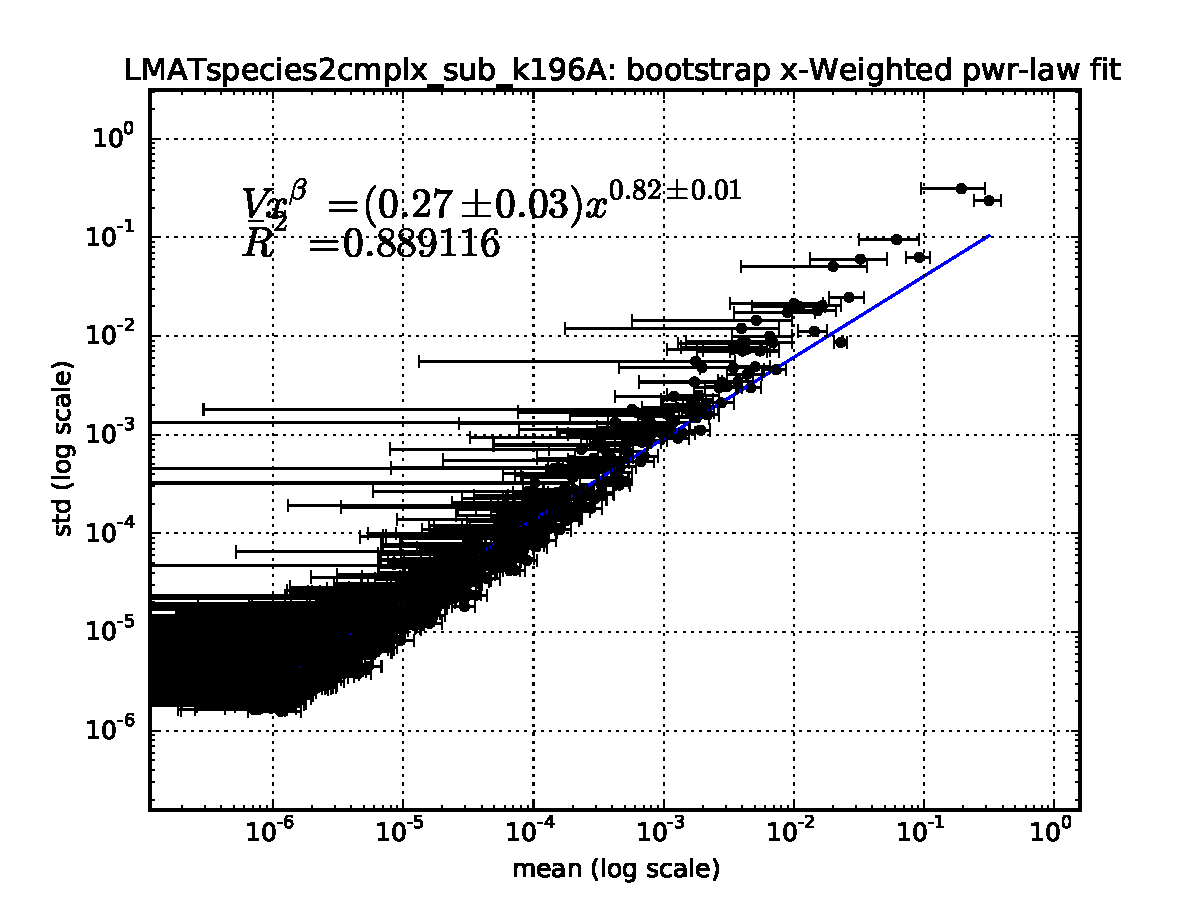
\includegraphics[width=0.5\textwidth]{results/taxalevel/xWb_spc_SMS.pdf}
\caption{Detail of comparison of different approaches based on adjacent taxonomic levels using plots of X-weighted power-law fits (see Material and Methods). The former row of subfigures shows examples for 16S, whereas the latter row of subfigures plots examples for SMS. The left column shows results for the superior taxonomic level (family for 16S, genus for SMS), while the right column shows results for the inferior level (genus for 16S, specie for SMS).}
\label{fig:taxlev2}
\end{figure}

%%
\subsection*{X-weighted power-law fit}\label{sec:X-w}

When fitting the power-law of std vs. mean, we can take into account that every mean has uncertainty and estimate it for a sample size $n$ by the SEM (\emph{Standard Error of the Mean}). Here, the uncertainties affect the independent variable, so the fit is not so trivial as a Y-weighted fit, where the uncertainties affect the dependent variable. A standard approach to do this fit is: a) invert your variables before applying the weights, b) then perform the weighted fit, and finally, c) revert the inversion. This method is deterministic, but the approximate solution worsens with smaller coefficients of determination. To overcome this limitation, we developed a stochastic method by using a bootstrapping-like strategy that avoids the inversion and is applicable regardless of the coefficient of determination. 

The basic idea of bootstrapping is that inference about a population from sample data (sample $\rightarrow$ population) can be modeled by resampling the sample data and performing inference on (resample $\rightarrow$ sample). To adapt this general idea to our problem, we resample the x-data array using its errors array. That is, for each replicate, a new x-data array is computed based on:
\begin{linenomath}
$$x^*_i = x_i + v_i$$
\end{linenomath}
where $v_i$ is a Gaussian random variable with mean $\mu_i=0$ and standard deviation $\sigma_i=\mathrm{SEM}_i$, as defined previously. For each replicate a complete un-weighted power-law fit is performed, where to choose between fitting power laws ($y=Vx^\beta$) using linear regression on log-transformed (LLR) data versus non-linear regression (NLR) we mainly follow \emph{General Guidelines for the Analysis of Biological Power Laws}\cite{ecology}. The parameters of the X-weighted fit are then estimated by averaging through all the replicate fits performed, and their errors are estimated by computing the standard deviation also for all the fits. At the end of each step, the relative error is calculated by comparing the fit parameters estimation in the last step with the previous one. Finally, both the coefficient of determination of the fit and the coefficient of correlation between the fit parameters are estimated by averaging.

%%
\subsection*{Rank Stability Index}\label{sec:RSI}

The Rank Stability Index (RSI) is shown as a percentage in a separate bar on the right of the rank matrix plot shown in Figure \ref{fig:corrank}. The RSI is strictly $1$ for an element whose range never changes over time, and is strictly $0$ for an element whose rank oscillates between the extremes from time to time. So, RSI is calculated, per element, as $1$ less the quotient of the number of true rank hops taken between the number of maximum possible rank hops, all powered to $p$:
\begin{linenomath}
$${\rm RSI} = \left(1-\frac{\text{true rank hops}}{\text{possible rank hops}}\right)^p = \left(1-\frac{D}{(N-1)(t-1)}\right)^p$$
\end{linenomath}
where $D$ is the total of rank hops taken by the studied element, $N$ is the number of elements that have been ranked, and $t$ is the number of time samples. The power index $p=4$ is arbitrarily chosen to increase the resolution in the stable region. 

The colour code of the RSI percentage text in the rank plot shown in Figure \ref{fig:corrank} is chosen following the first condition satisfied from those shown in Table \ref{tab:RSI}.

\begin{table}
  \begin{center}
    \begin{tabular}{cccr}
    \hline
    Case  &  Condition  &  Colour  &  Description \\
    \hline
    1  &  $1\ge{\rm RSI}>0.99$  & \textcolor{blue}{blue} & constant rank \\ 
    2  & ${\rm RSI}>0.90$  &  \textcolor{green}{green}  & highly stable rank \\
    3  &  ${\rm RSI}>0.75$  &  \textcolor{orange}{orange} & moderately stable rank \\
    4  &  ${\rm RSI}>0.25$  &  \textcolor{red}{red} & unstable rank \\
    5  &  $0.25\ge{\rm RSI}\ge0$  &  \bfseries{black} & very unstable rank \\
    \hline
    \end{tabular}
  \end{center} 
  \caption{Colour code of the RSI percentage text shown in Figure \ref{fig:corrank}, following the first condition satisfied.}
  \label{tab:RSI}
\end{table}

%%
\subsection*{Standardization} \label{sec:stan}
In order to properly show all the studies under common axes, we decided to standardize the Taylor parameters using the group of healthy individuals for each study. With this approach, all the studies can be visualized in a shared plot with units of Taylor-parameters standard-deviation on their axes.

For a Taylor parameter, e.g. $V$, the estimate of the mean ($\widehat{V}$) for the healthy subpopulation, composed of $h$ individuals, is:
\begin{linenomath}
$$\widehat{V} = \frac{1}{W_1}\sum_{i=1}^h V_i \omega_i=\sum_{i=1}^h V_i \omega_i$$
\end{linenomath}
as $W_1=\sum_i^h \omega_i=1$, since $\omega_i$ are normalized weights calculated as:
\begin{linenomath}
$$\omega_i = \frac{\frac{1}{\sigma^2_{V_i}}}{\sum_i^h\frac{1}{\sigma^2_{V_i}}}$$
\end{linenomath}
being $\sigma_{V_i}$ the estimation of the uncertainty in $V_i$ obtained together with $V_i$ from the X-weighted power-law fit described in Section \ref{sec:X-w}, for healthy individuals.

Likewise, the estimation of the standard deviation for the healthy population ($\widehat{\sigma}_V$) is:
\begin{linenomath}
$$\widehat{\sigma}_V = \sqrt{\frac{1}{W_1-\frac{W_2}{W_1}}\sum_{i=1}^h\left[\omega_i\left(V_i-\hat{V}\right)^2\right]}$$
\end{linenomath}
being $W_2=\sum_i^h \omega_i^2$, which finally yields to:
\begin{linenomath}
$$\widehat{\sigma}_V = \sqrt{\frac{1}{1-\sum_i^h \omega_i^2}\sum_{i=1}^h\left[\omega_i\left(V_i-\hat{V}\right)^2\right]}$$
\end{linenomath}
